%
% NOTE -- ONLY EDIT THE .Rnw FILE!!!  The .tex file is
% likely to be overwritten.
%
% Sweave("~/git/BioC2013/BioC2013_SS.Rnw")
% Stangle(system.file("BioC2013_SS.Rnw",package="ChipSeq"))
%\VignetteIndexEntry{}
% \VignetteDepends{PICS,rGADEM,MotIV,PING}
%\VignetteKeywords{}
%\VignettePackage{}

\documentclass[12pt]{article}

\usepackage{amsmath,pstricks}
% \usepackage[authoryear,round]{natbib}
\usepackage{hyperref}
\usepackage{amsmath}
\usepackage[super,numbers,round,sort&compress]{natbib}

\textwidth=6.2in
\textheight=8.5in
%\parskip=.3cm
\oddsidemargin=.1in
\evensidemargin=.1in
\headheight=-.3in

\newcommand{\scscst}{\scriptscriptstyle}
\newcommand{\scst}{\scriptstyle}


\newcommand{\Rfunction}[1]{{\textit{#1}}}
\newcommand{\Robject}[1]{{``#1''}}
\newcommand{\Rpackage}[1]{\texttt{#1}}
\newcommand{\Rmethod}[1]{\textit{#1}}
\newcommand{\Rfunarg}[1]{{`#1'}}
\newcommand{\Rclass}[1]{{\textit{#1}}}

\textwidth=6.2in

 
\usepackage{Sweave}
\begin{document}
%\setkeys{Gin}{width=0.55\textwidth}

\newtheorem{Exercise}{Exercise}[section]

\title{chip-seq data analysis \\ 2013 BioConductor LabSession: ``A Bioconductor pipeline for the analyis of ChIP-Seq experiments.''}
\author{Xuekui Zhang, Sangsoon Woo and Arnaud Droit}

\maketitle

\section{Introduction}

This package \Rclass{ChipSeq} provides all necessary data for the chip-seq sections of the 2013 BioConducor Labsession. This vignette also includes all commands that we will be used throughout the lab sessions \cite{Mercier:2011p5429,Zhang:2010p3139}.

\part{ChIP-Seq for Transcription Binding sites}
\section{Data Input}
For your convenience, the experimental data required in this package have already been pre-formatted and can simply be loaded with the following commands:
\begin{Schunk}
\begin{Sinput}
> library(ChipSeq)
> # Chip-seq ER data
> # This will load two datasets
> data(ER)
> # ChIP-Seq FOXA1 data
> data(FOXA1)
> # Mappability profiles
> data(mapp)
\end{Sinput}
\end{Schunk}

then the ER chip-seq data \cite{Hu:2010uq} will be loaded in your workspace and you can quickly have a look by typing
\begin{Schunk}
\begin{Sinput}
> ER.E2
\end{Sinput}
\begin{Soutput}
GRanges with 1682199 ranges and 8 metadata columns:
            seqnames                 ranges strand   |           id       run
               <Rle>              <IRanges>  <Rle>   | <BStringSet>  <factor>
        [1]     chr8 [121925697, 121925732]      -   |              20AC3AAXX
        [2]     chrX [ 62743396,  62743431]      +   |              20AC3AAXX
        [3]     chr3 [ 71521065,  71521100]      -   |              20AC3AAXX
        [4]     chr4 [152827245, 152827280]      +   |              20AC3AAXX
        [5]    chr17 [  6493232,   6493267]      -   |              20AC3AAXX
        ...      ...                    ...    ... ...          ...       ...
  [1682195]    chr19   [61458404, 61458439]      -   |              20AC3AAXX
  [1682196]    chr10   [41728199, 41728234]      +   |              20AC3AAXX
  [1682197]    chr14   [94534528, 94534563]      +   |              20AC3AAXX
  [1682198]     chr6   [36506343, 36506378]      +   |              20AC3AAXX
  [1682199]    chr19   [21059553, 21059588]      +   |              20AC3AAXX
                 lane      tile         x         y filtering   contig
            <integer> <integer> <integer> <integer>  <factor> <factor>
        [1]         5         1        11        93         N         
        [2]         5         1        12       761         N         
        [3]         5         1        14       482         N         
        [4]         5         1        15       525         N         
        [5]         5         1        16       814         Y         
        ...       ...       ...       ...       ...       ...      ...
  [1682195]         5       300       978       468         Y         
  [1682196]         5       300       982       435         N         
  [1682197]         5       300       984       722         N         
  [1682198]         5       300       986       431         N         
  [1682199]         5       300       988       556         Y         
  ---
  seqlengths:
    chr1 chr10 chr11 chr12 chr13 chr14 ...  chr7  chr8  chr9  chrM  chrX  chrY
      NA    NA    NA    NA    NA    NA ...    NA    NA    NA    NA    NA    NA
\end{Soutput}
\begin{Sinput}
> ER.ethl
\end{Sinput}
\begin{Soutput}
GRanges with 2322007 ranges and 8 metadata columns:
            seqnames                 ranges strand   |           id       run
               <Rle>              <IRanges>  <Rle>   | <BStringSet>  <factor>
        [1]     chr8 [ 25806295,  25806330]      -   |              20AC3AAXX
        [2]     chr4 [  6352505,   6352540]      -   |              20AC3AAXX
        [3]     chr8 [131650686, 131650721]      +   |              20AC3AAXX
        [4]    chr19 [ 16634246,  16634281]      -   |              20AC3AAXX
        [5]     chr7 [105529125, 105529160]      +   |              20AC3AAXX
        ...      ...                    ...    ... ...          ...       ...
  [2322003]     chr3 [142278087, 142278122]      +   |              20AC3AAXX
  [2322004]    chr14 [ 24370076,  24370111]      -   |              20AC3AAXX
  [2322005]     chr1 [ 67774697,  67774732]      +   |              20AC3AAXX
  [2322006]     chrX [ 76104833,  76104868]      +   |              20AC3AAXX
  [2322007]    chr15 [ 72428824,  72428859]      +   |              20AC3AAXX
                 lane      tile         x         y filtering   contig
            <integer> <integer> <integer> <integer>  <factor> <factor>
        [1]         3         1        14       472         N         
        [2]         3         1        21       215         Y         
        [3]         3         1        22        73         N         
        [4]         3         1        22       918         N         
        [5]         3         1        23       682         Y         
        ...       ...       ...       ...       ...       ...      ...
  [2322003]         3       227       606       881         Y         
  [2322004]         3       227       606       334         N         
  [2322005]         3       227       606       389         Y         
  [2322006]         3       227       607       643         N         
  [2322007]         3       227       607       649         Y         
  ---
  seqlengths:
    chr1 chr10 chr11 chr12 chr13 chr14 ...  chr7  chr8  chr9  chrM  chrX  chrY
      NA    NA    NA    NA    NA    NA ...    NA    NA    NA    NA    NA    NA
\end{Soutput}
\end{Schunk}
We have also included the raw data in the package, and the following commands should get you the pre-formatted data
\begin{Schunk}
\begin{Sinput}
> library(ShortRead)
> # ER data (Eland file)
> # Get the path of the data
> path <- system.file("extdata/chip-seq/ER",package = "ChipSeq")
> # Grep the treatment file
> E2.file<-list.files(path, pattern = "E2",full.names = FALSE)
> # Grep the control file
>  ethl.file<-list.files(path, pattern = "ethl",full.names = FALSE)
> # Set some filters
> filtChr<- chromosomeFilter("chr")
> filtUnique<-occurrenceFilter(min=1L, max=1L)
> filtStrand<-strandFilter(strandLevels=c("+","-"))
> filtOverall<-compose(filtChr,filtUnique,filtStrand)
> # Now we use ShortRead to read the data
>  ER.E2<-readAligned(path,type="SolexaExport",pattern=E2.file,filter=filtOverall)
>  ER.E2<- as(ER.E2, "GRanges")
> #Do the same for the IP file
>  ER.ethl<-readAligned(path,type="SolexaExport",pattern=ethl.file,filter=filtOverall)
>  ER.ethl<- as(ER.ethl, "GRanges")
> 
> 
> # save(ER.ethl,ER.E2,file="ER.rda")
\end{Sinput}
\end{Schunk}

\begin{Exercise}
Do the same process of generating GRanges object for FOXA1 chip-seq data.
\end{Exercise}


Here our aligned reads are stored in \Rclass{GRanges} objects whereas our mappability profiles are stored in \Rclass(RangedData} objects. Therefore we also change them to \Rclass{GRanges} objects. 
Note that the mappability profile is read length dependent. For each chromosome, a mappability profile for a specific read length (e.g. 36 bp) consists of a vector that lists an estimated read mappability `score' for each base pair in the chromosome. A score of one at a genomic position means that we should be able to uniquely align a read that overlaps that position, while a score of zero indicates that no read of that length should be uniquely alignable at that position. As noted above, typically only reads that map to unique genomic locations are retained for analysis. For convenience, and because transitions between mappable and non-mappable regions are often much shorter than the regions, we compactly summarize each chromosome's mappability profile as a disjoint union of non-mappable intervals that specify only zero-valued profile regions \\
 

\section{Statistical Analysis}
\subsection{Genome segmentation}

Because ChIP-seq aligned-read data are usually sparse, consisting largely of regions in which few or no reads are observed, we first preprocess the read data by segmenting the genome into regions, each of which has a minimum number of reads that aligned to forward and reverse strands. For computational efficiency, we recomend the utilization of the \Rpackage{parallel} package. We can set the number of cores for parellel computation by the argument of 'nCores'. By default the function uses only on core. Using the data we have read and formatted, as described above, we now use the \Rfunction{segmentPICS} function, as follows,
\begin{Schunk}
\begin{Sinput}
> data(ER)
> data(mapp)
> library(parallel)
> seg<-segmentPICS(ER.E2, dataC=ER.ethl, map=mapp36, minReads=1)
> summary(seg)
\end{Sinput}
\begin{Soutput}
** Experiment information ** 
Chromosomes interogated: chr1 chr10 chr11 chr12 chr13 chr14 chr15 chr16 chr17 chr18 chr19 chr2 chr20 chr21 chr22 chr3 chr4 chr5 chr6 chr7 chr8 chr9 chrM chrX chrY 
Number of reads in IP:  1682199  and in control:  2322007 
** Segmentation parameters ** 
The following settings were used:
  Sliding window half width:  250 
  Step size:  20 
  Minimum number of reads:  1 
** Segmentation summary ** 
Number of segmented regions: 11566 
Summary on the number of Forward/Reverse reads per region:
  Forward:
     Min. 1st Qu.  Median    Mean 3rd Qu.    Max. 
   3.00    4.00    6.00   12.19   12.00 1440.00 
  Reverse:
     Min. 1st Qu.  Median    Mean 3rd Qu.    Max. 
   3.00    4.00    6.00   12.28   12.00 1492.00 
Summary on the number of control Forward/Reverse reads per region:
  Forward:
     Min. 1st Qu.  Median    Mean 3rd Qu.    Max. 
    0.0     0.0     1.0     4.6     2.0  2990.0 
  Reverse:
      Min.  1st Qu.   Median     Mean  3rd Qu.     Max. 
   0.000    0.000    1.000    4.631    2.000 3073.000 
** Mappability summary **
Non mappable intervals cover an average  0.07630552 % of all regions 
\end{Soutput}
\end{Schunk}

the returned value is a \Rclass{segReadsList} object. Each element of the \Rclass{segReadsList} contains the reads for the corresponding `candidate' region as well as the mappability intervals intersecting the region.
 
\subsection{Data smoothing and PICS processing:}
Now that we have created our seg object, we are ready to fit \Rfunction{PICS} to each region, this is automatically done with the \Rfunction{PICS} function.

\begin{Schunk}
\begin{Sinput}
> # This might take about a few minutes on a single cpu, but we can set the number of cores for the parrelel run. 
> pics<-PICS(seg, nCores=2)
\end{Sinput}
\end{Schunk}
\noindent\textbf{The \Rclass{picsList} object and accessors:} 
The object returned by the \Rfunction{PICS} function is an S4 class containing all necessary information (e.g. parameters, scores, etc). We have implemented numerous accessors for you to efficiently retrieve important information from such an object. All of them are documented in the \Rfunction{PICS} vignette, available with the package, but we review a few important accessors here:
\begin{Schunk}
\begin{Sinput}
> #Get the location of the binding sites (mid-point of the motifs).
> mu<-mu(pics)
> # Get the fragment length estimates from all binding events
> delta<-delta(pics)
> summary(delta)
\end{Sinput}
\begin{Soutput}
   Min. 1st Qu.  Median    Mean 3rd Qu.    Max. 
-1376.0   133.9   161.7   162.2   188.9  1402.0 
\end{Soutput}
\begin{Sinput}
> # Get the enrichment score from all binding events
> score<-score(pics)
> summary(score)
\end{Sinput}
\begin{Soutput}
   Min. 1st Qu.  Median    Mean 3rd Qu.    Max. 
  0.000   2.233   4.141   8.181   8.282 188.400 
\end{Soutput}
\end{Schunk}

These are simple vectors containing all estimated parameters across candidate regions, and one can see that the average fragment size distributions is about 144 bps. In order to better visualize the fragment length estimates across binding events, we can use a simple histogram.
\begin{Schunk}
\begin{Sinput}
> # For clarity, we focus on (0,500)
> hist(delta,xlim=c(0,500),50,main="Average fragment length distribution")
\end{Sinput}
\end{Schunk}
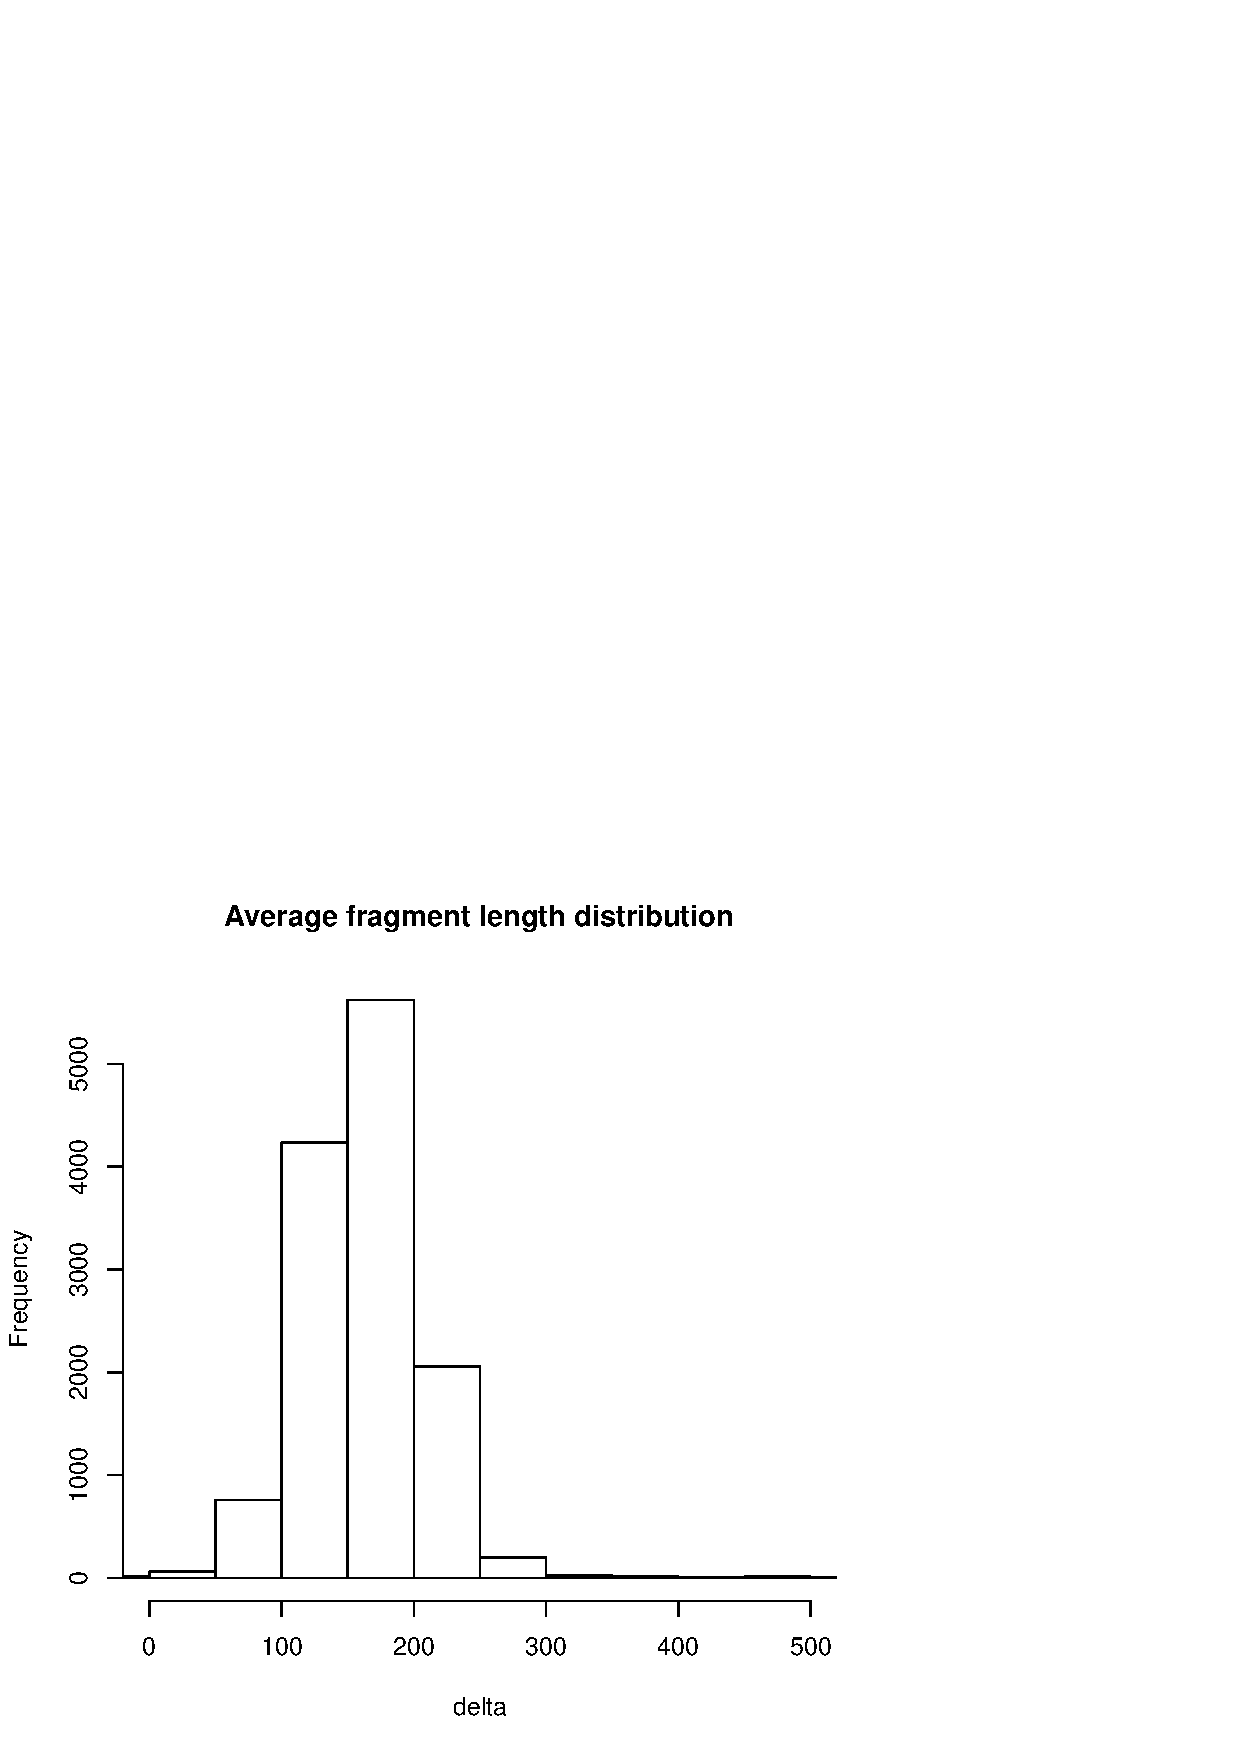
\includegraphics{chipData_AD-PICS-fragment-length-distribution}

In \Rpackage{PICS}, each candidate region (a list element of seg) can contain multiple binding sites, and to summarize the number of events/region we can use the \Rmethod{K} accessor which will give us the number of binding events estimated for each region.
\begin{Schunk}
\begin{Sinput}
> # Retrieve the number of events per region
> nEvents<-K(pics)
> # Tabulate these numbers
> table(nEvents)
\end{Sinput}
\begin{Soutput}
nEvents
    0     1     2     3     4     5     6     7     8 
  116 10108  1110   195    31     2     1     1     2 
\end{Soutput}
\end{Schunk}
We have also included a simple plotting method for visualizing a candidate region with the PICS estimated parameters, as follows,

\begin{Schunk}
\begin{Sinput}
> plot(pics[2],seg[2])
\end{Sinput}
\end{Schunk}
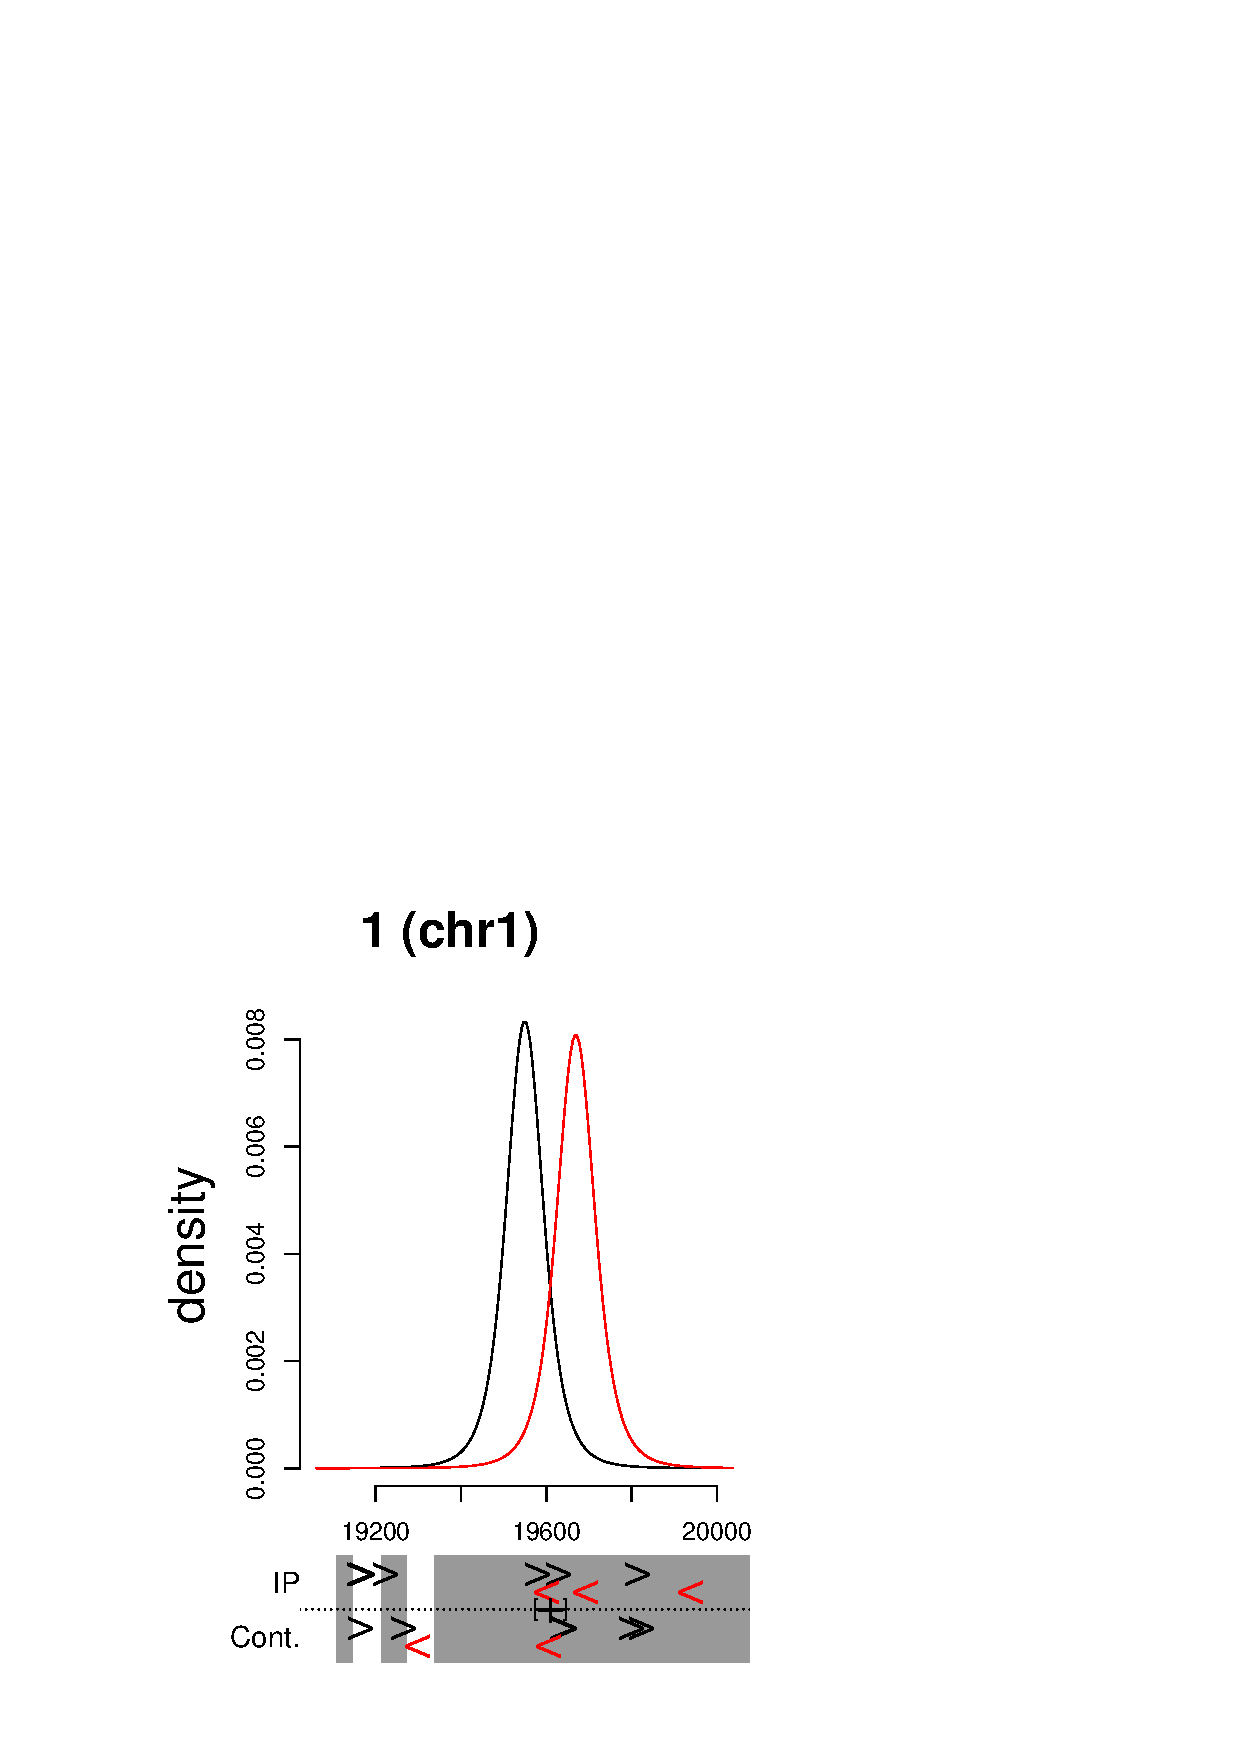
\includegraphics{chipData_AD-PICS-plots}

\subsection{Detecting enriched regions:}
The next step would consist of selecting a list of estimated binding events to be prioritized for further analysis (e.g. motif analysis, or correlation with annotations). In the absence of control data, this needs to be done arbitrarily. For example, one could want to focus on all regions that have an enrichment score greater than 4. This can simply be done when exporting our \Robject{pics} object to a \Rclass{RangedData} object, as follows, with the appropriate filter

\begin{Schunk}
\begin{Sinput}
> # Filter atypical peaks
> myFilter<-list(score=c(1,Inf),delta=c(50,300),se=c(0,50),sigmaSqF=c(0,22500),sigmaSqR=c(0,22500))
> # Make a RangedData Object
> RD<-makeRangedDataOutput(pics, type="bed",filter=myFilter) 
> library(rtracklayer)
> export(RD, "myfile.bed")
\end{Sinput}
\end{Schunk}

where we used the type bed for export, other export types (e.g. wig, fixed, etc) are also available. Please refer to the PICS vignette and man pages for more details.
Note that above, we only keep the binding events that have a score greater than 4, a delta value (average fragment length) between 50 and 300, and standard deviation (strand specific peak width) less than 150 ($150^2=22500$). 
If one wishes to export all events with typical filters (and score>1), we provide a shortcut with the \Rmethod{as} method as follows:
\begin{Schunk}
\begin{Sinput}
> RD<-as(pics,"RangedData")
\end{Sinput}
\end{Schunk}
similarly if one wishes to export all events as a \Rclass{data.frame} with all PICS parameters without filtering, we can use
\begin{Schunk}
\begin{Sinput}
> DF<-as(pics,"data.frame")
\end{Sinput}
\end{Schunk}
The \Rfunction{makeRangedDataOutput} can also be used to produce a `wig' type track with base level scores, as follows,
\begin{Schunk}
\begin{Sinput}
> # Filter atypical peaks
> myFilter<-list(score=c(1,Inf),delta=c(50,300),se=c(0,50),sigmaSqF=c(0,22500),sigmaSqR=c(0,22500))
> # Make a RangedData Object
> RDwig<-makeRangedDataOutput(pics, type="wig",filter=myFilter)
\end{Sinput}
\begin{Soutput}
[1] "Removing overlapping binding events"
\end{Soutput}
\begin{Sinput}
> export(RDwig, "myfile.wig")
\end{Sinput}
\end{Schunk}


\subsection{FDR calculation}
In the presence of the control, it is possible to generate an FDR curve that can be used to select an appropriate threshold. The first step is to rerun the same analysis after swapping the control and IP samples, as follows:
\begin{Schunk}
\begin{Sinput}
> segC<-segmentPICS(data=ER.ethl, dataC=ER.E2, map=mapp36, minReads=1)
> picsC<-PICS(segC, nCores=2)
> fdr <- picsFDR(pics, picsC, filter=list(delta=c(50, Inf), se=c(0,50), sigmaSqF=c(0, 22500), sigmaSqR=c(0, 22500)))
\end{Sinput}
\end{Schunk}
note that we have created a method for plot. If you input two pics objects, an FDR curve will be generated. \textbf{Note that the second argument needs to be the control.}
\begin{Schunk}
\begin{Sinput}
> plot(pics,picsC)
\end{Sinput}
\end{Schunk}
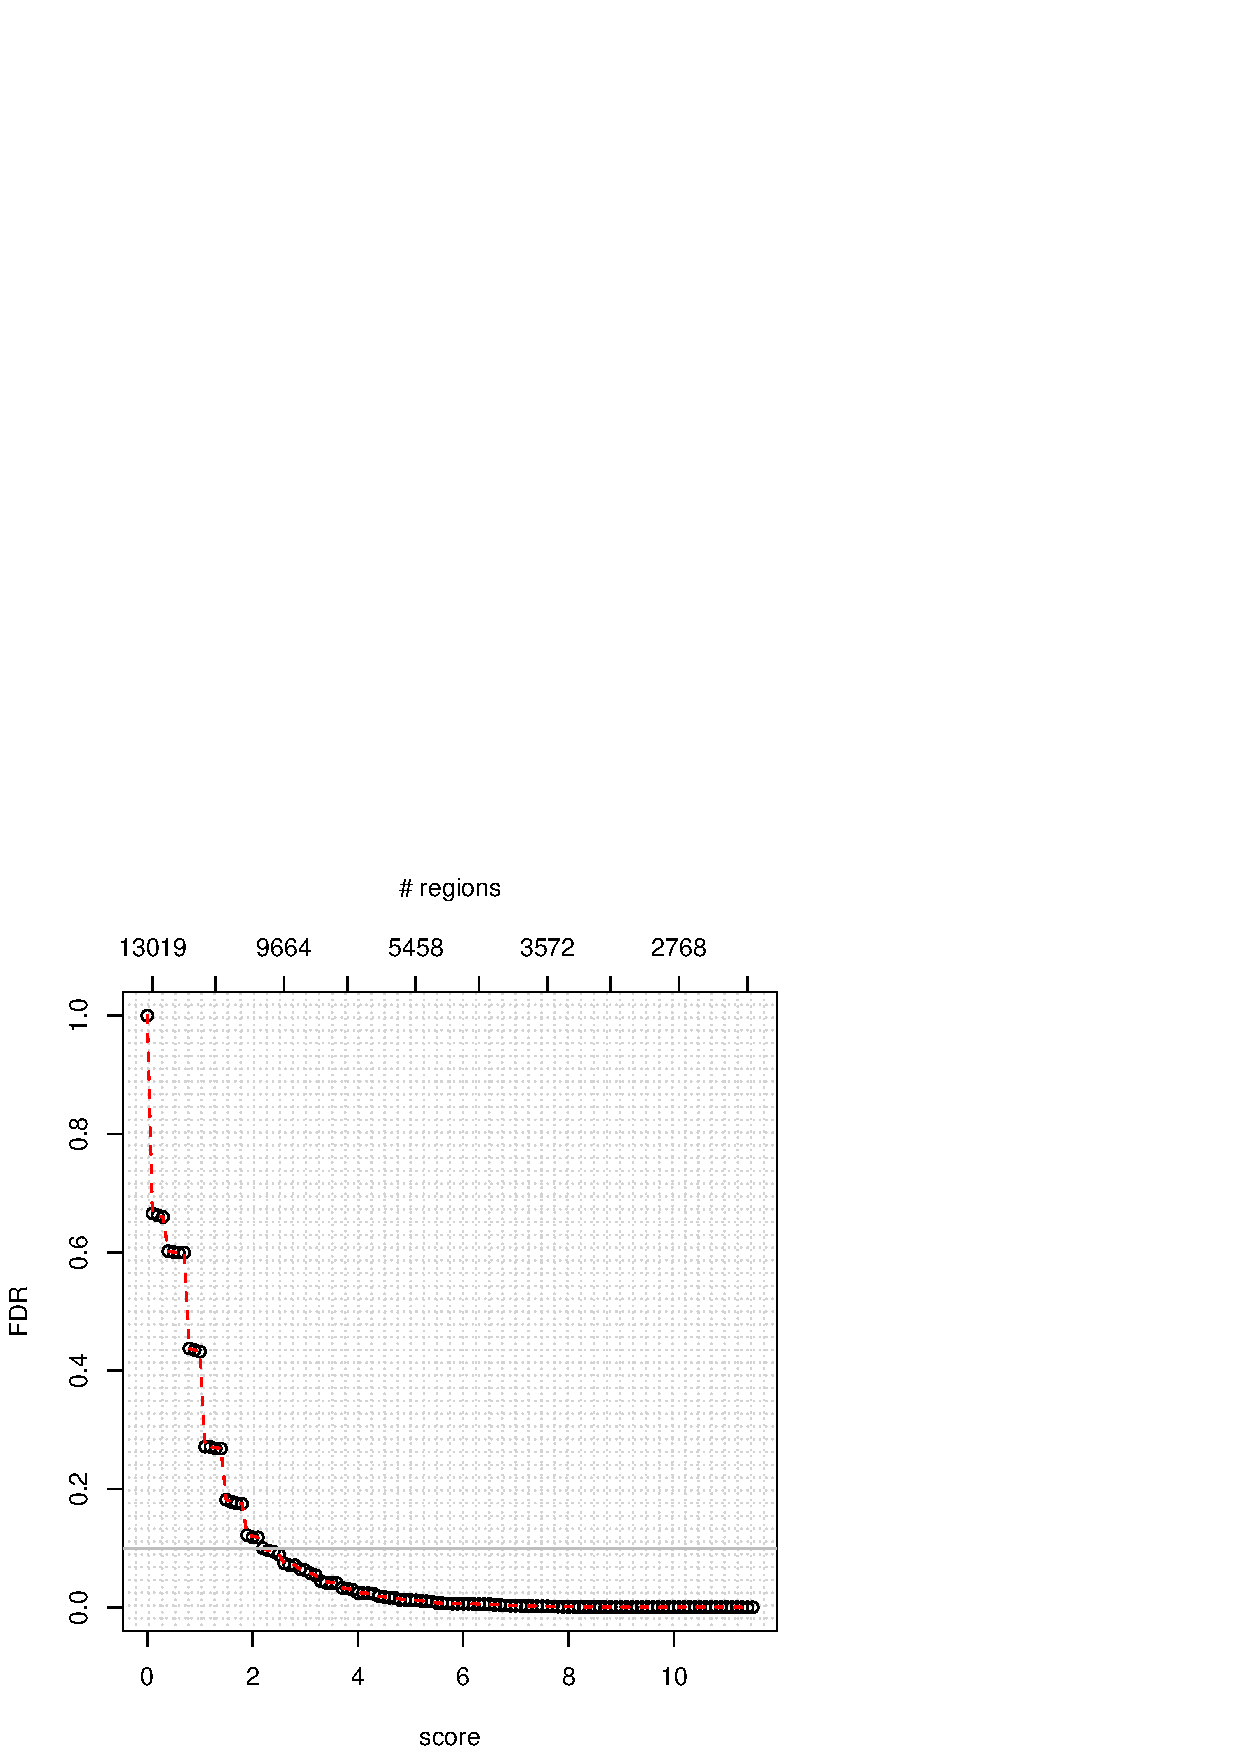
\includegraphics{chipData_AD-PICS-FDR}
and one can see that a threshold score of 2 would lead to an estimated FDR of about 10\% with about 300 regions
If we want to use a score of 2 as threshold and filter atypical regions we can simply use

\begin{Schunk}
\begin{Sinput}
> # Filter atypical peaks
> myFilter<-list(score=c(2,Inf),delta=c(50,300),se=c(0,50), sigmaSqF=c(0,22500),sigmaSqR=c(0,22500))
> # Make a RangedData Object
> RD<-makeRangedDataOutput(pics, type="bed", filter=myFilter)
\end{Sinput}
\end{Schunk}
We can also visualize the FDR as a functioin fo the number of regions.


\section{Visualization}
The visualization of enriched regions and track lines is possible thanks to \Rpackage{GenomeGraphs} and \Rpackage{rtracklayer}.
We first explore the \Rpackage{GenomeGraphs} package. In the example below, we will graph our enriched regions in a subset of chromosome 21 along with the nearest genes, 
\begin{Schunk}
\begin{Sinput}
> library(GenomeGraphs)
> # Here I use the current genome build
> mart = useMart("ensembl", dataset = "hsapiens_gene_ensembl")
> genomeAxis<-makeGenomeAxis(add53 = TRUE, add35 = TRUE)
> RDwig1<-RDwig["chr21"]
> RD1<-RD["chr21"]
> minbase<-start(RD1[2,])-500
> maxbase<-start(RD1[2,])+500
> genesplus<-makeGeneRegion(start = minbase, end = maxbase, strand = "+",
+  chromosome = 21, biomart = mart) 
> genesmin<-makeGeneRegion(start = minbase, end = maxbase, strand = "-", 
+ chromosome = 21, biomart = mart)
> score = makeBaseTrack(value=score(RDwig1), base = start(RDwig1), 
+ dp = DisplayPars(lwd=2,color="black", type="h"))
> rectList<- makeRectangleOverlay(start = start(RD1), end = end(RD1), 
+ region = c(1, 4), dp = DisplayPars(color = "green", alpha = 0.1))
> gdPlot(list("score" = score, "Gene +" = genesplus, Position = genomeAxis, 
+ "Gene -" = genesmin), minBase = minbase, maxBase = maxbase, labelCex = 1,
+ overlays=rectList)
\end{Sinput}
\end{Schunk}
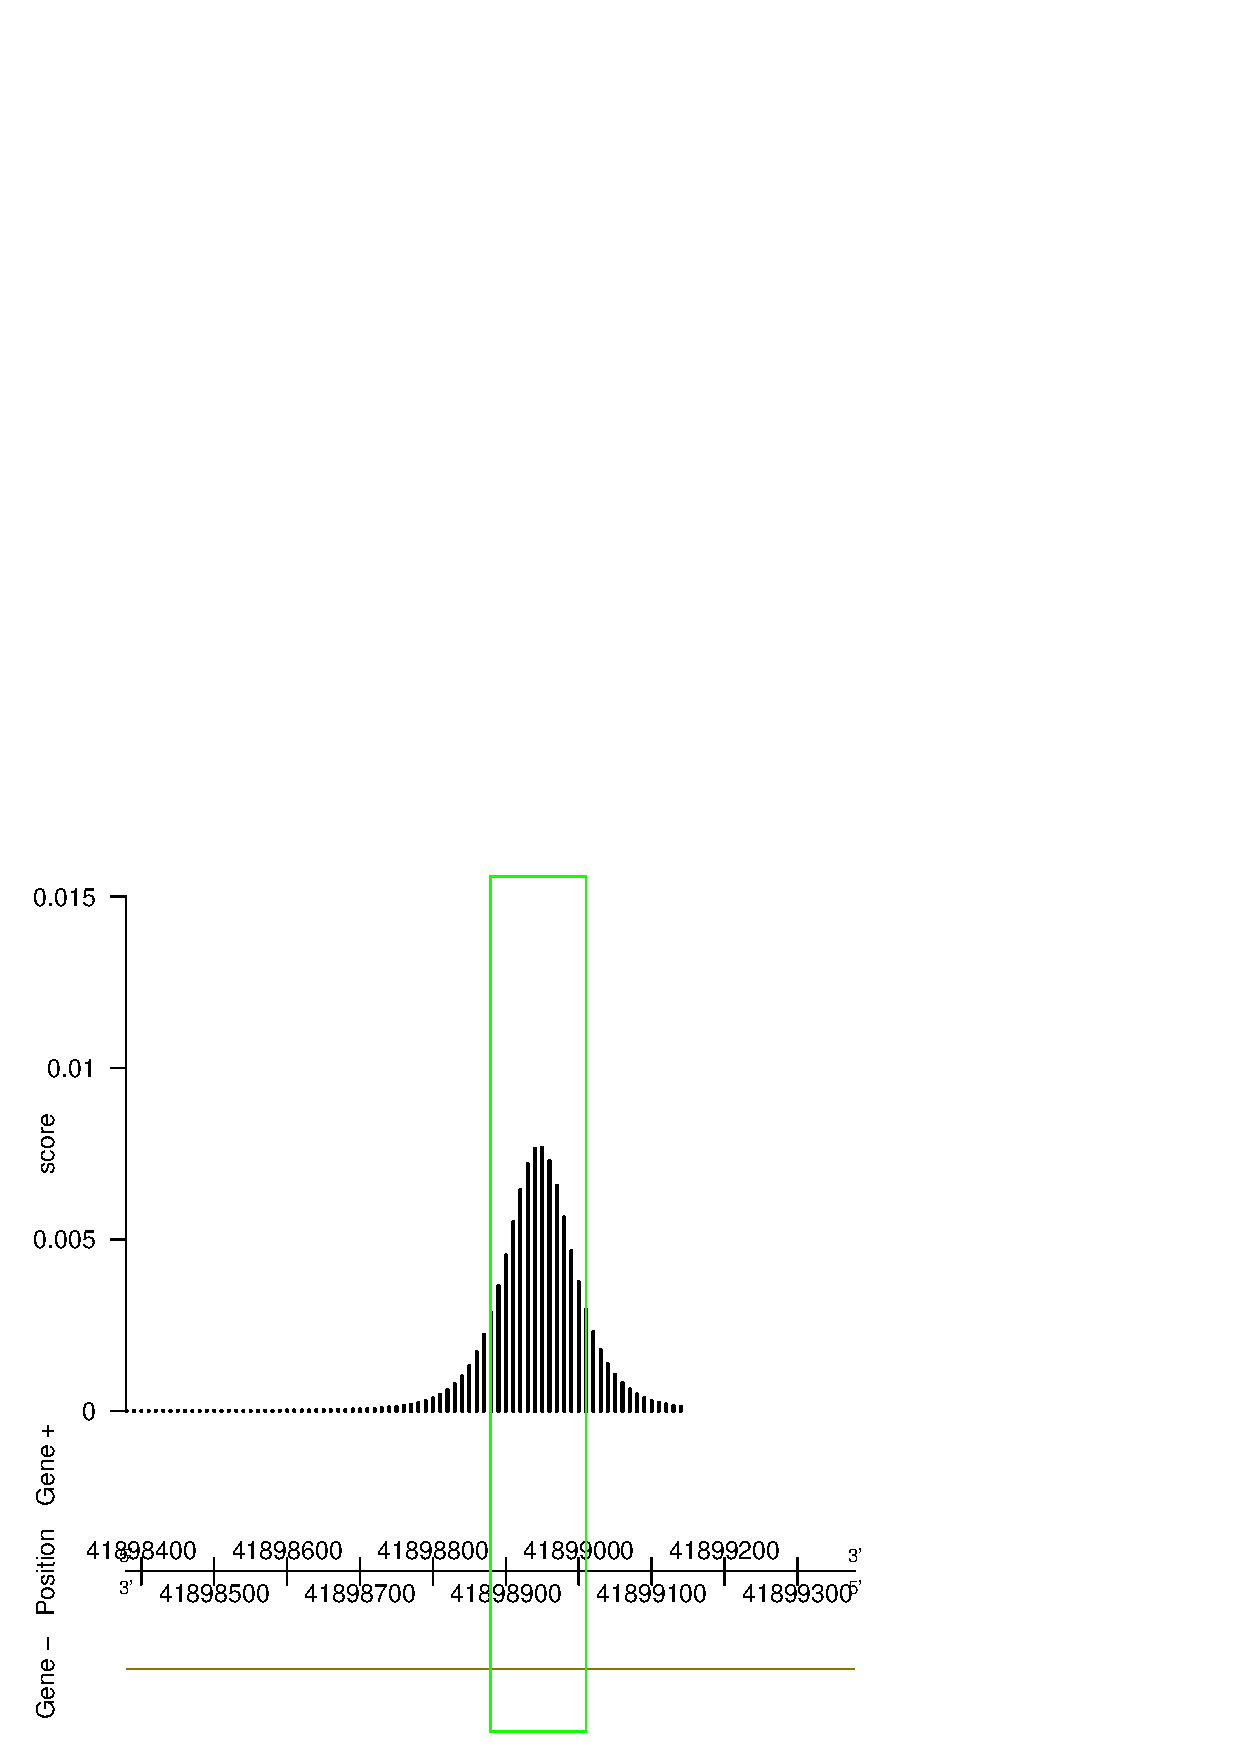
\includegraphics{chipData_AD-Visualization-GenomeGraphs-cs}

Now we look at the \Rpackage{rtracklayer} package. \Rpackage{rtracklayer} is basically allowing us to interact with the UCSC genome browser directly from R. 
\begin{Schunk}
\begin{Sinput}
> library(rtracklayer)
> ## start a session
> RD_GR<-as(RD,"GRanges")
> session <- browserSession("UCSC")
> track(session, "targets") <- RD_GR
> subtrack<-RD_GR[2]
> view <- browserView(session, subtrack * -10, pack = c("Conservation","RepeatMasker"))
\end{Sinput}
\end{Schunk}

Of course, you always have the option to export the results as wig/bed and load it in your favorite browser. Export functionalities are also provided by the \texttt{rtracklayer} package.

\begin{Schunk}
\begin{Sinput}
> library(rtracklayer)
> # These functions are provided by rtracklayer
> export(RD,"ERregions.bed")
> export(RDwig,"ERscore.wig")
\end{Sinput}
\end{Schunk}

\section{De Novo motif discovery:}
After having detected enriched regions, it is common to perform sequence analysis to detect biologically 
relevant motifs that can be used to validate our regions and/or to gain novel insights about the biology of gene regulation. In collaboration with Leiping Li, we have developed an R package specifically designed to work on large set of sequences typically return by a ChIP-Seq experiment. \Rpackage{rGADEM} combines spaced dyads and an expectation-maximization (EM) algorithm. Candidate words (four to six nucleotides) for constructing spaced dyads are prioritized by their degree of overrepresentation in the input sequence data. Spaced dyads are converted into starting position weight matrices (PWMs). \Rpackage{rGADEM} then employs a genetic algorithm (GA), with an embedded EM algorithm to improve starting PWMs, to guide the evolution of a population of spaced dyads toward one whose entropy scores are more statistically significant. Spaced dyads whose entropy scores reach a pre specified significance threshold are declared motifs. 
Here we will perform a motif analysis of the set of ER enriched regions returned by PICS using an FDR of 10\%

\begin{Schunk}
\begin{Sinput}
> library(rGADEM)
> library(BSgenome.Hsapiens.UCSC.hg18)
> RDfixed<-makeRangedDataOutput(pics, type="fixed")
> RDfixed_top100<-RDfixed[1:100,]
> ERgadem<-GADEM(RDfixed_top100,seed=1,genome=Hsapiens,verbose=TRUE)
> # save(ERgadem,file="ERgadem.rda")
\end{Sinput}
\end{Schunk}

Now we will post-process and visualize our regulatory motifs using the package \Rpackage{MotIV}. \Rpackage{MotIV} is similar to STAMP \cite{Mahony:2007p125} with added graphics functionalities. It allows you to compare your identified motifs to known motifs according to some database (e.g. Jaspar\cite{PortalesCasamar:2010p543}) and report the best matches. \Rpackage{MotIV} includes the Jaspar database and will use it by default, however you are free to use your own, please refer to the vignette of the \Rpackage{MotIV} for more details.

\begin{Schunk}
\begin{Sinput}
> library(MotIV)
> data(ERgadem)
> # Find the 5 best match in Jaspar.
> jaspar.match <- motifMatch(inputPWM = getPWM(ERgadem), top = 5)
\end{Sinput}
\begin{Soutput}
	Ungapped Alignment
	Scores read
	Database read
	Motif matches : 5
\end{Soutput}
\begin{Sinput}
> # Plot the motifs with their matches
> plot(jaspar.match , main = "Motifs in ER",top=5)
\end{Sinput}
\end{Schunk}
\includegraphics{chipData_AD-MotIV-cs}
\begin{Schunk}
\begin{Sinput}
> library(MotIV)
> data(ERgadem)
> # Find the 5 best match in Jaspar.
> jaspar.match <- motifMatch(inputPWM = getPWM(ERgadem), top = 5)
\end{Sinput}
\begin{Soutput}
	Ungapped Alignment
	Scores read
	Database read
	Motif matches : 5
\end{Soutput}
\begin{Sinput}
> # Plot the motifs with their matches and distribution
> plot(jaspar.match , ERgadem,main = "Motifs in ER")
\end{Sinput}
\end{Schunk}
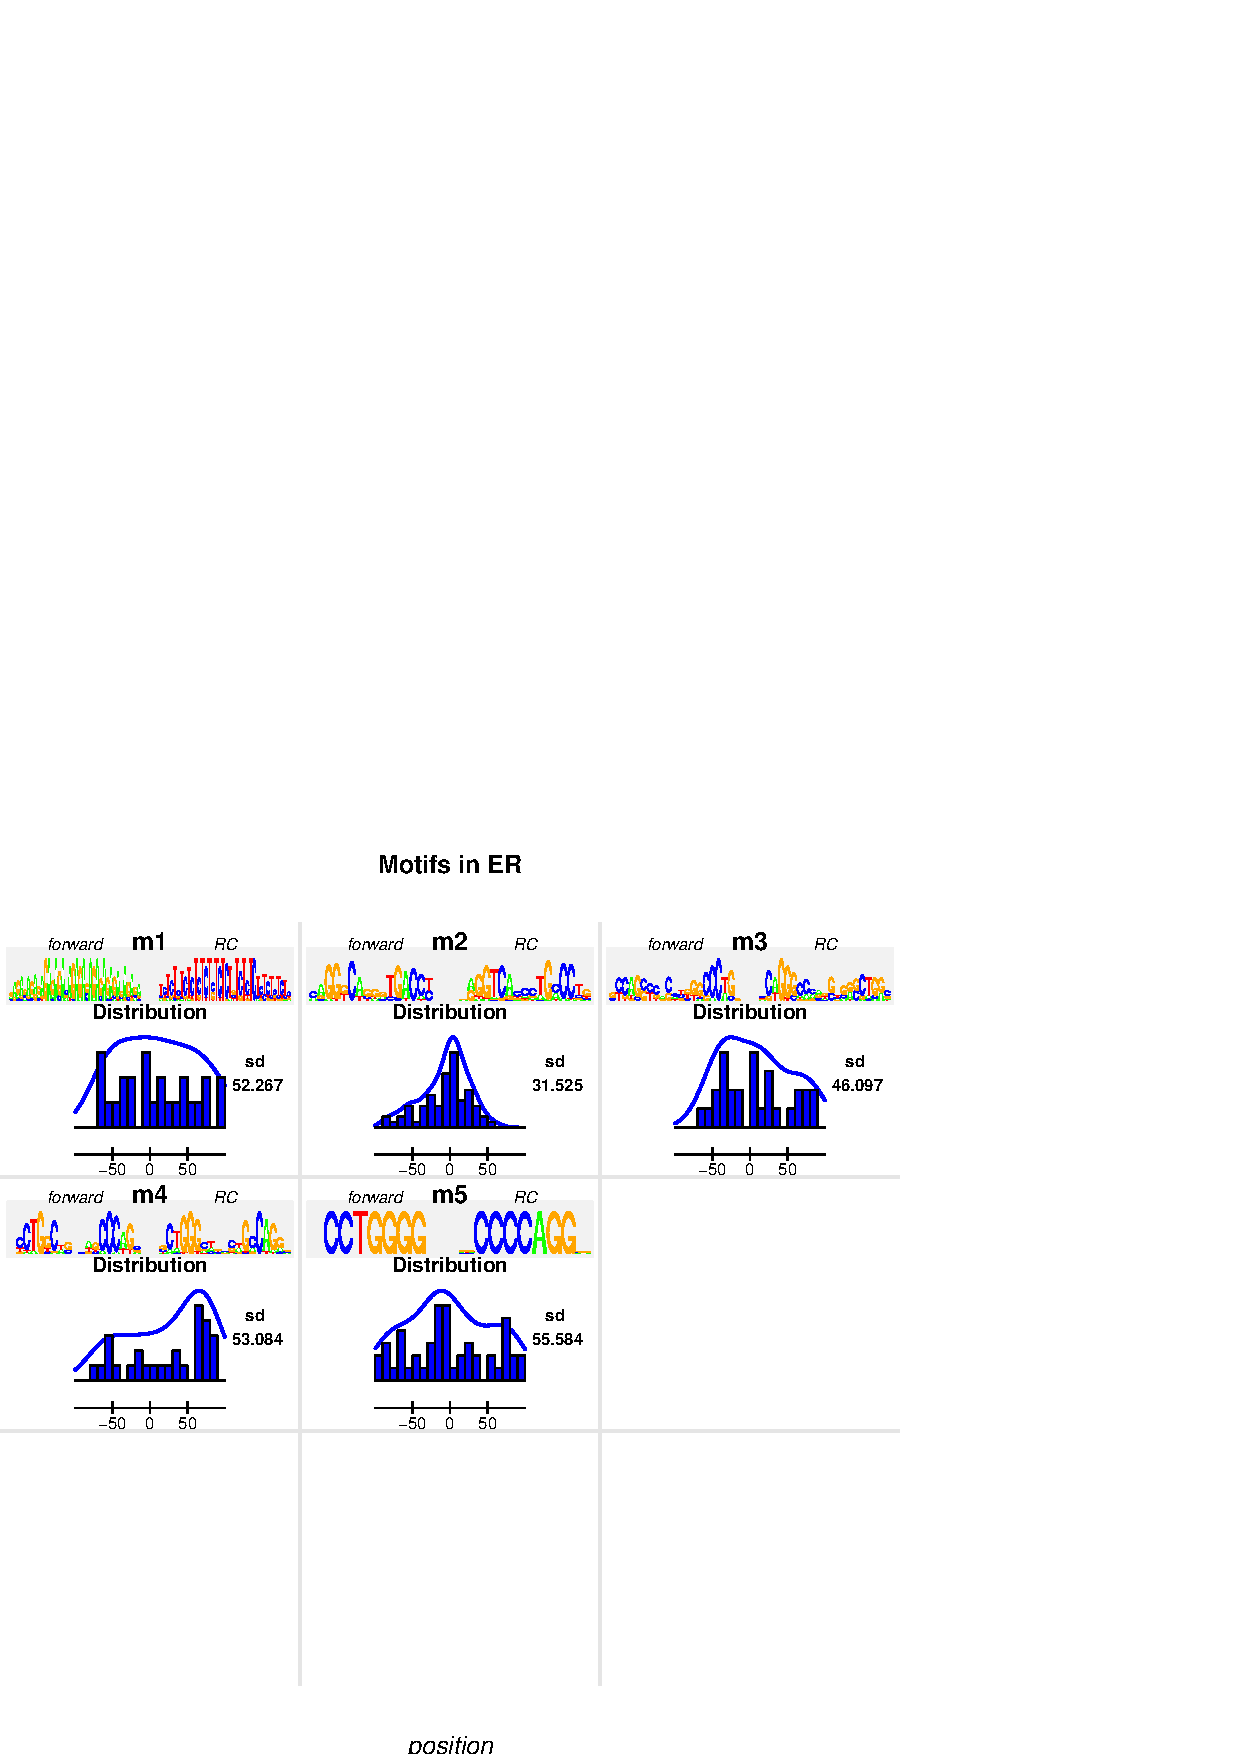
\includegraphics{chipData_AD-MotIV-cs2}

When rGADEM identifies multiple motifs, visualization and validation can become difficult. \Rpackage{MotIV} allows the user to filter motifs based on a set of filters. This is done with the function \Rfunction{setFilter}, as follows,
\begin{Schunk}
\begin{Sinput}
> Filter<-setFilter(name = "", tfname = "ESR1", top = 5, evalueMax = 10^-4)
> jaspar.match.ESR1<-filter(jaspar.match, Filter, verbose = TRUE)
> plot(jaspar.match.ESR1 , main = "ER motif",top=5)
> ERoc<-exportAsRangedData(jaspar.match.ESR1, ERgadem, correction=TRUE)
\end{Sinput}
\end{Schunk}
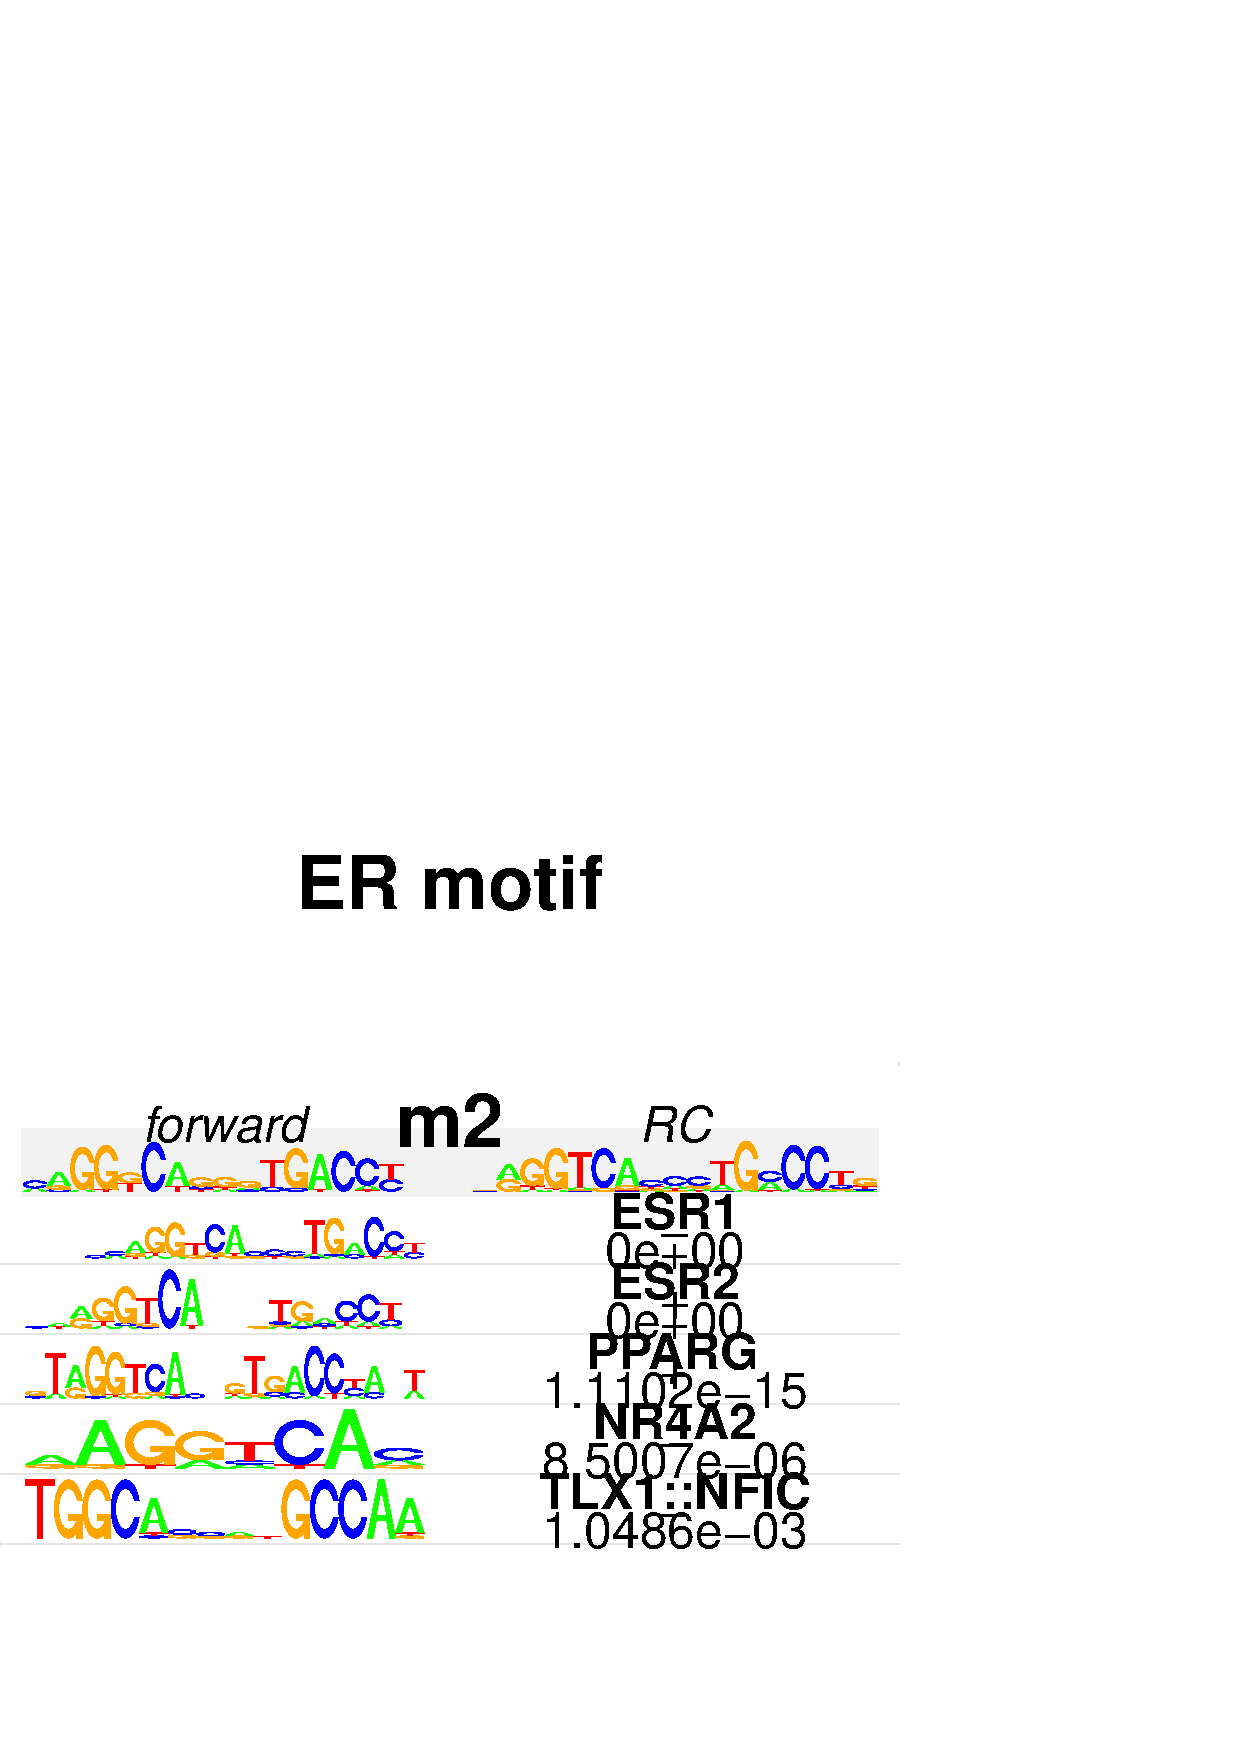
\includegraphics{chipData_AD-Filtering-with-MotIV}

rGADEM provides an option where the algorithm is initialized using a known motif, we refer to this option as a seeded analysis. Seeded analysis can be of particular use for short motifs and/or noisy data (e.g. Chip-chip) where a regular (unseeded) analysis might be more difficult. In the code snippet below, we use the ESR1 Jaspar motif as our seed.

The ER is included in the Jaspar database (named ESR1).
\begin{Schunk}
\begin{Sinput}
> # Normalize the PSSM -> PWM
> ERpwm<-apply(jaspar[["ESR1"]],2,function(x){x/sum(x)})
> # Make a PWM object that can be plotted with seqLogo
> library(seqLogo)
> ERpwmLogo<-makePWM(ERpwm)
> 
\end{Sinput}
\end{Schunk}

\includegraphics{chipData_AD-ESR1-motif-in-Jaspar-cc}

\begin{Schunk}
\begin{Sinput}
> # Seeded analysis
> library(rGADEM)
> library(BSgenome.Hsapiens.UCSC.hg18)
> RDfixed<-makeRangedDataOutput(pics, type="fixed", filter=myFilter)
> RDfixed_top100<-RDfixed[1:100,]
> ERgadem<-GADEM(RDfixed_top100,genome=Hsapiens,pValue=5*10^-6,minSites=5, 
+ Spwm=list(ERpwm,ERpwm,ERpwm,ERpwm,ERpwm,ERpwm,ERpwm,ERpwm))
\end{Sinput}
\end{Schunk}

Note that seeded runs are typically faster than unseeded ones. Now, we once again analyze the results using MotIV,
\begin{Schunk}
\begin{Sinput}
> jaspar.match <- motifMatch(inputPWM = getPWM(ERgadem), top = 5)
\end{Sinput}
\begin{Soutput}
	Ungapped Alignment
	Scores read
	Database read
	Motif matches : 5
\end{Soutput}
\begin{Sinput}
> plot(jaspar.match , main = "Motifs in ER data", top=5)
\end{Sinput}
\end{Schunk}
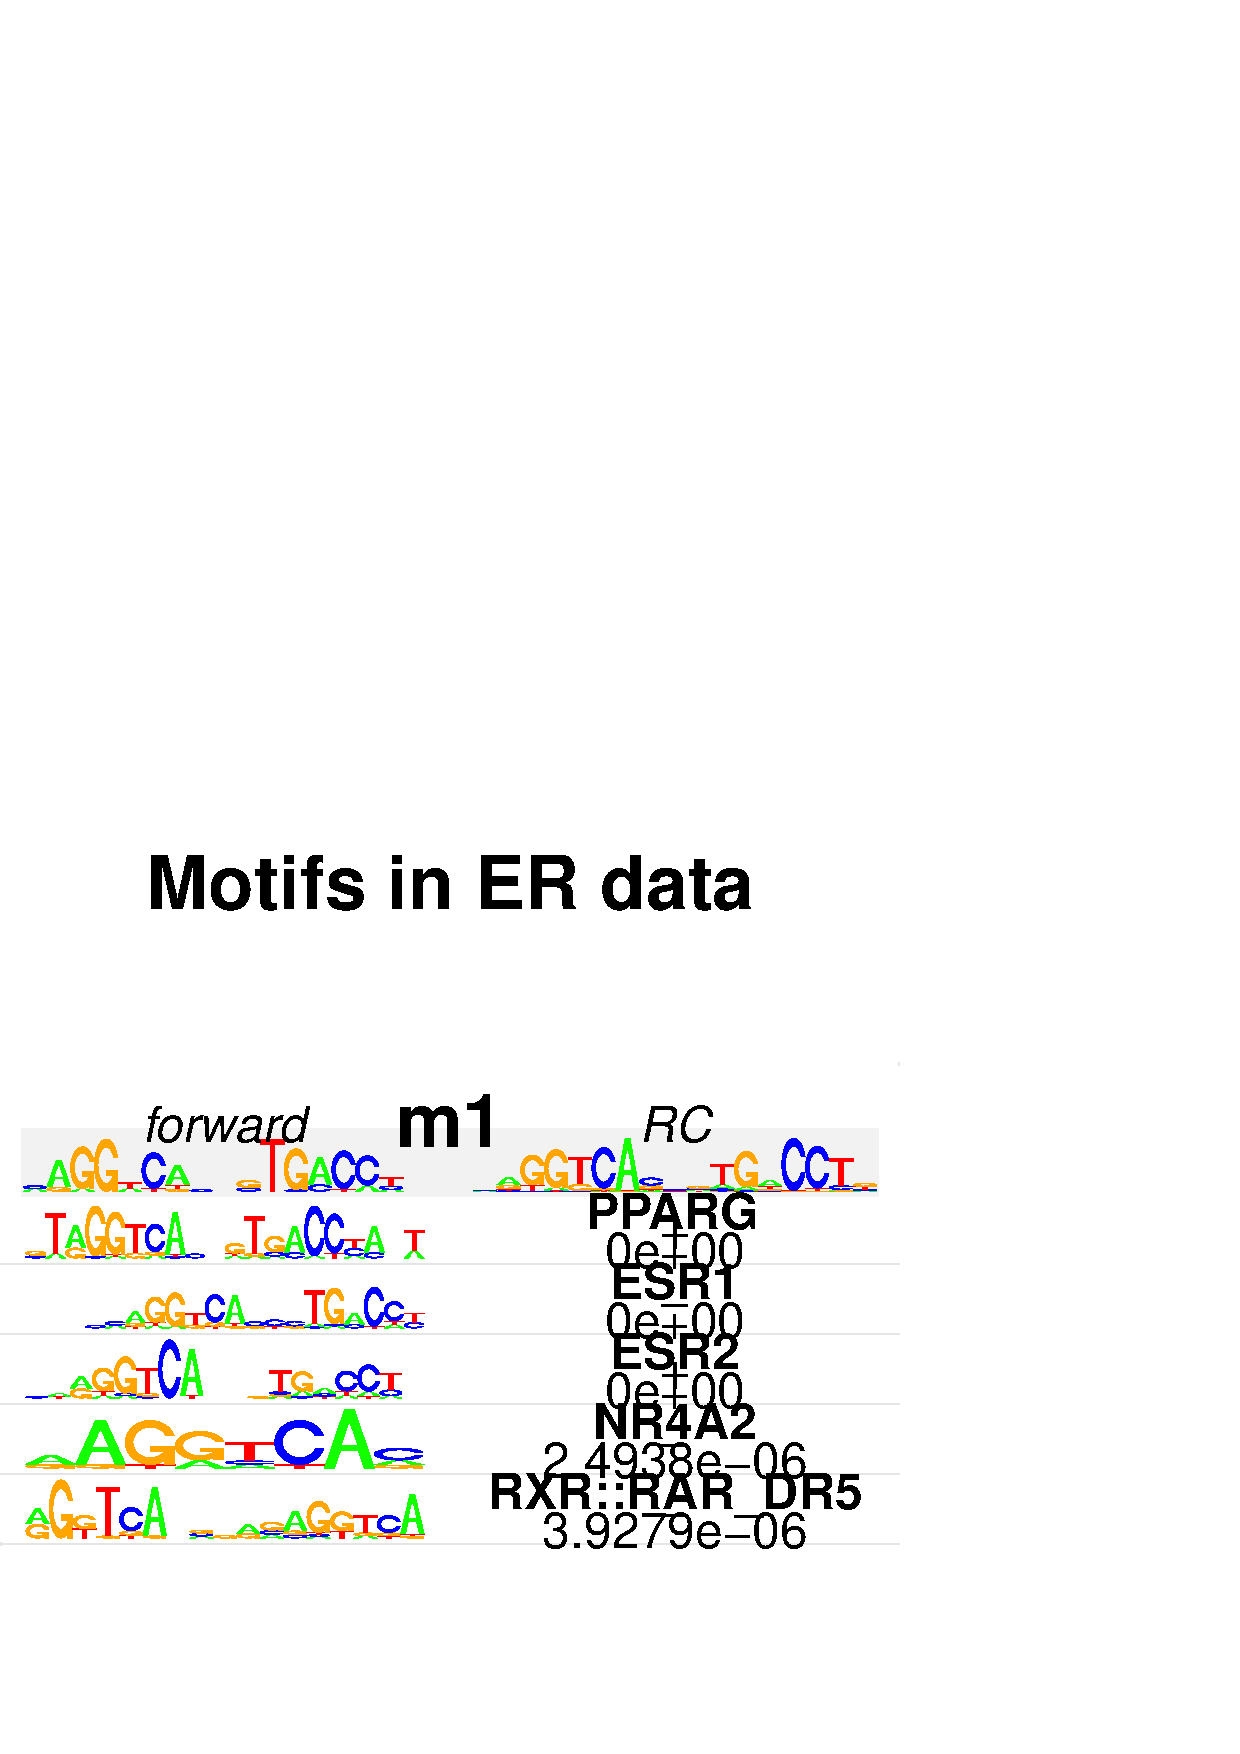
\includegraphics{chipData_AD-MotIV-seeded-cc}

and we can see that one motif has been selected based on its match to the ESR1 Jaspar motif.
\begin{Exercise}
Try the above with a different eValue filter and/or motif name.
\end{Exercise}

\section{Annotation of enriched regions:}
Here we explore the package \Rpackage{ChIPpeakAnno}\cite{Zhu:2010fk}, a package that facilitates the batch annotation of the peaks identified from either ChIP-seq or ChIP-chip experiments. Using \Rpackage{ChIPpeakAnno} you can find the nearest gene, exon, miRNA or custom features supplied by users such as most conserved elements and other transcription factor binding sites leveraging the \Rpackage{IRanges} package. 
Here we load the TSS NCBI36 coordinates and look at possible possible overlaps with our ER binding sites. The \Rfunction{annotatePeakInBatch} will do that for you and in addition will compute the distance to the closest feature (here TSS).
\begin{Schunk}
\begin{Sinput}
> library(ChIPpeakAnno)
> data(TSS.human.NCBI36)
> annotatedPeak <- annotatePeakInBatch(ERoc, AnnotationData = TSS.human.NCBI36)
> # Plot the distances to TSS
> hist(annotatedPeak$distancetoFeature,50)
\end{Sinput}
\end{Schunk}
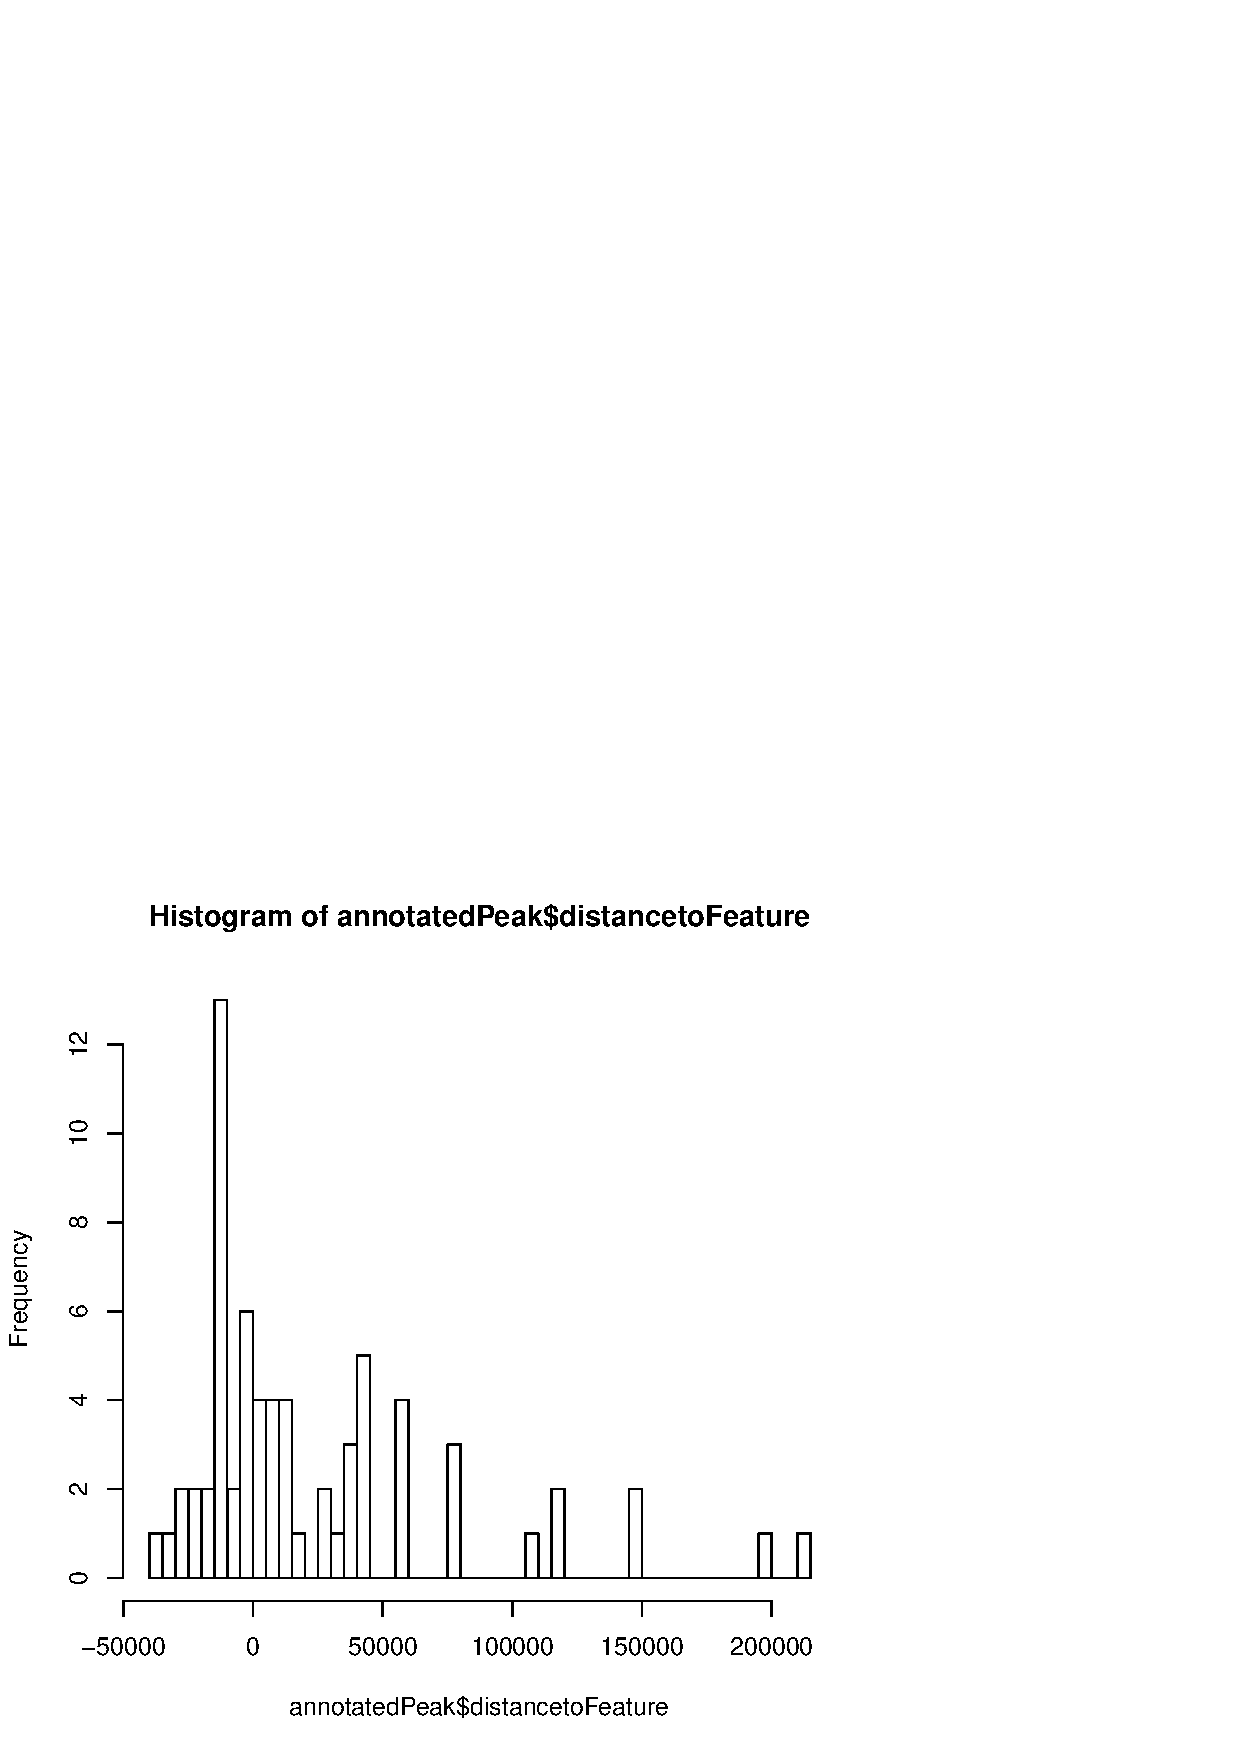
\includegraphics{chipData_AD-ChIPpeakAnno}


\begin{Exercise}
Use the \Rpackage{rtracklayer} package to plot the motif occurrences.
\end{Exercise}


\begin{Exercise}
Perform the same analysis with the FOXA1 data.
\end{Exercise}



\begin{Schunk}
\begin{Soutput}
	Ungapped Alignment
	Scores read
	Database read
	Motif matches : 5
\end{Soutput}
\end{Schunk}


\part{MNase-Seq and ChIP-Seq for Nucleosome positioning}
\section{Introduction}
The nucleosome is the basic structural unit of chromatin, which is composed of a nucleosomeal core including $147$bp of DNA wrapped around a central histone octamer (H2A, H2B, H3 and H4) and `linker` DNA connecting nucleosomal core to the next. Because limited accessibility, identifying nucleosome positioning helps biologists to understand the cellular mechanism. The \Rclass{PING} package is develpped for identifying nucleosome positioning. 
  
\section{Data Input}
The package is developped for single-end and also paired-end sequencing ChIP-Seq data.  
The basic data input of \Rclass{PING} is a \Rclass{GRanges} objects condtaining the directional aligned reads(SE data) or recondtructed DNA fragments(PE data). \Rclass{GRanges} can be derived from `BED` and `BAM` formats. 

\begin{Schunk}
\begin{Sinput}
> library(PING)
> library(ShortRead)
> # SE data (Single-End data file)
> # Get the path of the data
> path <- system.file("extdata/chip-seq/SE",package = "ChipSeq")
> SE<-read.table(file.path("SE.bed"), header=TRUE)
> SE<- as(SE, "GRanges")
\end{Sinput}
\end{Schunk}
\begin{Exercise}
Do convert data `SE.bam` to \Rclass{GRanges} object.
\end{Exercise}


The \Rlass{PICS} package includes \Rfunction{bam2gr} function for converting a `BAM` format to \Rclass{GRanges} object.

\begin{Exercise}
Do convert data `SE.bam` to \Rclass{GRanges} object. 
\end{Exercise} 


\section{Statistical Analysis}
\subsection{Genome segmentation}
Because of sparseness of the ChIP-Seq data, we pull out genomic regions including a minimum number of forward and reverse reads. We use \Rfunction{segmentPING} function for calling candidate regions. However, the regions including nuclesomes are usually wider than those including transcription binding sites. Therfore, we set some filtering arguments in \Rfunction{segmentPING} as following:

\begin{Schunk}
\begin{Sinput}
> seg<-segmentPICS(data=SE, minReads=NULL, maxLregion=1200, minLregion=80, jitter=TRUE)
> summary(seg)
\end{Sinput}
\end{Schunk}

For \Rclass{PING}, the returned value is also a \Rclass{segReadsList} object. Each element of the \Rclass{segReadsList} contains the reads for the corresponding `candidate' region as well as the mappability intervals intersecting the region.


\subsection{PING processing:}
Now that we have created our `seg` object, we are ready to use\Rfunction{PING} to probabilitically detect positioned nucleosomes.  

\begin{Schunk}
\begin{Sinput}
> ping<-PING(seg, nCores=2)
\end{Sinput}
\end{Schunk}

The \Rclass{PING} is for MNase and sonicated data sets. Therefore, the user should know which datatype they are dealing with. All default parameters are set for `MNase` datatype. In order to use `sonicated` data, the user should add the argument `dataType` in the function. The warning message states whether the parameters are set for `MNase` datatype or `sonicated` one.

\noindent\textbf{The \Rclass{pingList} object and accessors:}
The returned object from the \Rfunction{PING} function is an S4 class containing all necessary information (e.g. parameters, scores, etc). We have implemented numerous accessors for you to efficiently retrieve important information from such an object. All of them are documented in the \Rfunction{PING} vignette, available with the package, but we review a few important accessors here:
\begin{Schunk}
\begin{Sinput}
> #Get the location of the binding sites (mid-point of the motifs).
> mu<-mu(ping)
> # Get the fragment length estimates from all binding events
> delta<-delta(ping)
> summary(delta)
> # Get the enrichment score from all binding events
> score<-score(ping)
> summary(score)
\end{Sinput}
\end{Schunk}

For visualization of the estimated fragment lengths, we can simply use histgram. The estimated fragment length of the data is around $147$ bp, which is very close to the DNA framgnet size wrapping around a nucleosome.
 
\begin{Schunk}
\begin{Sinput}
> hist(delta,xlim=c(0,500),50,main="Average fragment length distribution")
\end{Sinput}
\end{Schunk}

\subsection{Pose-processing PING results}

The variation in nucleosome-based short-read data lead that some of PING's predictions may be inaccurate. For example, when a nucleosome with strong signal is adjacent to nucleosomes with weaker signals, \Rclass{PING} may fit two forward mixture componets and one reverse component. This causes a mismatch of forward/reverse peaks of other nucleosomes. We need to detect and resolve such problematic regions using \Rfunction{postPING} function.The argument of `dataType` in both \Rfunction{PING} and \Rfunction{postPING} should be consistent.

\begin{Schunk}
\begin{Sinput}
> PS <- postPING(ping, seg)
\end{Sinput}
\end{Schunk}

The output of \Rfunction{postPING} is a dataframe including all estimated parameters for each identified nucleosome position. The user can use \Rfunction{write.table} function to export the result. 

\begin{Exercise}
Export the postPING result.
\end{Exercise}

\subsection{Export result}

For further analysis including uploading the identified nucleosome positions in `UCSC` browser, we use the \Rfunction{makeRangedDataOutput} to export \Rclass{pingList} from \Rfunction{PING} or the \Rclass{data.frame} from \Rfunction{postPING} to different data formats. 

\begin{Schunk}
\begin{Sinput}
> ## Exporting PING result 
> rdBed <- makeRangedDataOutput(ping, type="bed")
> library(rtracklayer)
> export(rdBed, file="ping.bed")
\end{Sinput}
\end{Schunk}

The function uses the estimated fragment size in the `BED` format to infer the ranges where as the 'fixed' type is a `BED` format with a fixed nucleosome size of $147$bp.  

\begin{Exercise}
Export the postPING result using `fix` type.
\end{Exercise}



\subsection{Visualization}

To faciliate with the \Rclass{Gviz} package, the user can visualize the identified nucleosome positions for a given ranges. The \Rclass{PING} also includes a built-in plotting function \Rfunction{ploSummary}. 

\begin{Schunk}
\begin{Sinput}
> plotSummary(PS, ping, SE, "chr1", "gen", from=149000, to=153000)
\end{Sinput}
\end{Schunk}

The plot shows the predicted nucleosome positions, the associated score for each nucleosome and the profile of the short reads in addition to the alighned reads. The user can filter the nucleosomes passing some threshold of the score using the argument of \Rclass{scoreThreshold}. We also can hide the score track on the graph by setting the argumet of \Rclass{scoreTrack} as `FALSE`

\begin{Exercise}
Replot the predicted nucleosome positions for the same genomic region without score track.
\end{Exercise}


The user also can use functions in \Rclass{Gviz} to customize their own plot. The available functions for creating tracks in the \Rclass{PING} package are \Rfunction{CoverageTrack}, \Rfunction{RawReadsTrack}, and \Rfunction{NucleosomeTrack}

\begin{Schunk}
\begin{Sinput}
> library(Gviz)
> cTrack <- CoverageTrack(ping, dataIP, "chr1", "gen")
> rTrack <- RawReadsTrack(ping, dataIP, "chr1", "gen", name = "Reads")
> nTrack <- NucleosomeTrack(PS, "chr1", "gen", scoreThreshold = 0.1, name = "NEW")
> ## Add genomic information using Gviz's built-in functions. 
> gTrack <- GenomeAxisTrack(add53 = TRUE, add35 = TRUE)
> aTrack <- AnnotationTrack(start = 149500, end = 151000, showFeatureId= TRUE,
+      id = "random annotation", col.title = "orange", chr = "chr1",
+      gen = "gen", name = "custom")
> plotTracks(trackList = c(gTrack, cTrack, aTrack, rTrack, nTrack),
+      main = "Custom plot", from = 149000, to = 153000)
\end{Sinput}
\end{Schunk}

\end{document}



\section{Session Info}
\begin{Schunk}
\begin{Sinput}
> sessionInfo()
\end{Sinput}
\begin{Soutput}
R Under development (unstable) (2013-05-01 r62700)
Platform: x86_64-apple-darwin12.3.0 (64-bit)

locale:
[1] fr_CA.UTF-8/fr_CA.UTF-8/fr_CA.UTF-8/C/fr_CA.UTF-8/fr_CA.UTF-8

attached base packages:
[1] grid      parallel  stats     graphics  grDevices utils     datasets 
[8] methods   base     

other attached packages:
 [1] ChIPpeakAnno_2.9.4                  GenomicFeatures_1.13.17            
 [3] limma_3.17.16                       org.Hs.eg.db_2.9.0                 
 [5] GO.db_2.9.0                         RSQLite_0.11.4                     
 [7] DBI_0.2-7                           AnnotationDbi_1.23.16              
 [9] BSgenome.Ecoli.NCBI.20080805_1.3.17 multtest_2.17.0                    
[11] Biobase_2.21.6                      VennDiagram_1.6.0                  
[13] BSgenome.Hsapiens.UCSC.hg18_1.3.19  GenomeGraphs_1.21.0                
[15] biomaRt_2.17.2                      rtracklayer_1.21.8                 
[17] ChipSeq_1.0.0                       MotIV_1.17.0                       
[19] rGADEM_2.9.0                        seqLogo_1.27.0                     
[21] BSgenome_1.29.0                     GenomicRanges_1.13.27              
[23] Biostrings_2.29.13                  XVector_0.1.0                      
[25] IRanges_1.19.15                     PICS_2.3.01                        
[27] BiocGenerics_0.7.2                 

loaded via a namespace (and not attached):
 [1] bitops_1.0-5      lattice_0.20-15   MASS_7.3-26       RCurl_1.95-4.1   
 [5] Rsamtools_1.13.22 splines_3.1.0     stats4_3.1.0      survival_2.37-4  
 [9] tools_3.1.0       XML_3.98-1.1      zlibbioc_1.7.0   
\end{Soutput}
\end{Schunk}

\bibliographystyle{unsrt}
\bibliography{chipData_AD}

\end{document}
